\chapter{Structural Risk Minimization}
\label{ch:structuralriskminimization}\index{structuralriskminimization|(}


Structural Risk Minimization (SRM) is a technique first developed in 1974 by \citet{vapnikchervonenkis1}, used to identify the function $f(x)$ that solves a machine learning problem $y=f(x)$. SRM attempts to find a balance between training the model as accurately as possible, while not having an overly complex solution.
\newline
Consider the equation below \citep{srmvapnik512}:

\begin{equation}\label{srm1}
\centering
\min_{f}{\left[\hat{R}(f)+\epsilon(f)\right]}
\end{equation}
\newline
The first part of this equation is the training loss, or what we can refer to as the expected risk $\hat{R}(f)$. The expected risk is found based on the training data, and represents the frequency of errors on our training set. Parameters are adjusted to minimize $\hat{R}(f)$ so as to obtain the best possible model for our problem. This technique is referred to as Empirical Risk Minimization (ERM). The second part of the equation $\epsilon(f)$ refers to the capacity measure of the function. This is used to quantify the complexity of our function $f$.

\section {VC-Dimension} \label{sec:vc-dimension}\index{structuralriskminimization!vc-dimension}

A vital topic for one to be able to understand SRM is the VC-Dimension. The theory about uniform convergence of empirical risk to actual risk describes various conditions, as well as the bounds for the rate of convergence. These bounds are based upon a measure of the capacity of the set of functions implemented by the model, also known as the VC-Dimension \citep{srmvapnik506}. Before looking at the definition of the VC-Dimension, it is important to understand the following definition:

\newtheorem{definition}{Definition}
\begin{definition} \label{shatterdefn}
Given a collection $F$ of subsets of a set $S$, we say that the finite subset $A$ of $S$ is shattered provided that every subset $B$ contained in $A$ can be written as intersection of $A$ with an element of $F$. 
\end {definition}
The VC-Dimension is defined\citep{srmvapnik506} as:
\begin{definition} \label{vcdimdefn}
The VC-dimension of a set of indicator functions is the maximum number $h$ of vectors that can be shattered in $2^{h}$ ways by using functions within that set. 
\end {definition}
It should be noted that a VC-Dimension of $h$ does not mean that all sets of $h$ points can be shattered by a given set of functions, but there is at least one example of it occurring.


\section {Structural Risk Minimization} \label{sec:srm}

Suppose $m$ is the size of our sample, and $h$ is our VC dimension. When $\frac{m}{h}$ is large enough, our VC confidence is negligible and hence, it can be ignored and ERM can take place. However, when $\frac{m}{h}$ is small, the VC confidence can no longer be ignored. When this is the case, we need to be able adjust the VC-dimension $h$ of our model \citep{srmvapnik506}. This is where Structural Risk Minimization comes in. It is a technique that allows a trade off in accurate model fitting and avoiding overcomplexity. One may think that we would want our VC-dimension $h$ to be a high value, as our risk $R(f)$ drops. However, while this is true, this would increase the chances of overfitting. This is why we have our complexity term $\epsilon$, as it increases when this occurs. On the other hand, if $h$ is too low, then we would have an issue of our $R(f)$ being too high. So the user must have the right balance of accuracy and complexity.
\newline
In mathematical terms, SRM is carried out by first selecting a family of classifiers $\{F(x,w)\}$, and then defining a structure of nested subsets of the elements of the family: $S_{1}\subset S_{2}\subset\ldots\subset S_{n-1}\subset S_{n}$, where $S_{i}=\left\{ f(x,w),\:w\in W_{i}\right\} $. Due to the structure of the subsets, their respective VC-dimension satisfies: $h_{1}<h_{2}<\ldots<h_{n-1}<h_{n}$. Our goal is to find the optimal structure for our problem, denoted $S^{*}$.
\newline
\newline
To find this optimal structure, we carry out the following steps, as described by \citet{srmvapnik506} and \citet{srmsewell}:

\begin{enumerate}
\item Find the ERM for each element of the structure $\hat{f_{i}}=\mathrm{arg\,\underset{\mathnormal{f}\in \mathnormal{S_{i}}}{min}}\hat{R}(f)$
\item Next we calculate $i_{*}={\mathrm{{arg\,\underset{\mathnormal{i}\in\mathbb{N}}{min}}}}R(\hat{f_{i}})+\epsilon_{i}$
and return $f_{i_{*}}$
\end{enumerate}

A loss function $L(f(x),y)$ is used to represent our risk function $\hat{R}(f)$, of which there are many examples, such as the hinge loss function or the $\epsilon$-insensitive loss function, used in support vector regression. This function calculates the gap between the function $f(x)$ used as our solution, and the output $y$. \newline
The generalization error of our function, $\epsilon(f)$, is a more technical proposition, explained below using the theorems \ref{Th:srmthm1} and \ref{Th:srmthm2} described by \citet{shawetaylorsrm}. These theorems are used to provide an upper bound for $\epsilon(f)$ with confidence $1-\delta$. This is a very important result for us, as while we want our loss function $L(f(x),y)$ to be as small as possible, it is important that $\epsilon(f)$ is not too high. 
\newline
$\mathrm{Er}_{\mathbf{z}}(s)$ is the number of errors that $s$ makes on $z$. $\mathrm{er}_{\mu}(s)$ represents the expected error, based on probability measure $\mu$, when $x_1,\dots,x_m$ are drawn independently.

\newtheorem{srmtheorem}{Theorem}
\begin{srmtheorem} \label{Th:srmthm1}
Let $0<\epsilon<1$ and $0<\gamma\leq1$ Suppose S is a hypothesis space of functions mapping the input space $X$ to $\left\{0,1\right\}$, and let $\mu$ be any probability measure on $G=X\times\left\{0,1\right\}$. The probability with respect to $\mu^m$ that for some $\mathbf{z}\in G^m$, $\exists s \in S$ s.t. $\mathrm{er}_{\mu}(s)>\epsilon$ and $\mathrm{Er}_{\mathbf{z}}(s)\leq m(1-\gamma)\mathrm{er}_{\mu}(s)$, that is at most:
\begin{equation}\label{srmeqn1}
4\Pi_{S}(2m)\mathrm{exp}\left(-\frac{\gamma^2\epsilon m}{4}\right)
\end{equation}
\end{srmtheorem}

Theorem \ref{Th:srmthm1} is used to prove theorem \ref{Th:srmthm2}, shown below. $p_{d}$ represents the probability that $S_d$ is the smallest class containing a consistent hypothesis. On the other hand, $q_{dk}$ represents the probability of errors in the training set. It influences the trade off between the selected function's complexity and accuracy.

\begin{srmtheorem} \label{Th:srmthm2}
Let $S_{1},S_{2},\ldots$ be a sequence of hypothesis classes mapping {X} to $\left(0,1\right)$ and having VC-dimension $i$. Let $\mu$ be any probability measure on $S=X\times\left(0,1\right)$, and let $p_d$, $q_dk$ be any sets of positive numbers satisfying 
\begin{equation}\label{srmeqn2}
\displaystyle \sum_{d=1}^{\infty} p_{d} = 1
\end{equation}
and $\sum_{k=0}^{m} q_{dk} = 1$ for all $d$. Then with probability $1-\delta$ over $m$ independent identically distributed examples $x$, if the learner finds a hypothesis $f$ in $S_d$ with $Er_{x}(f)=k$, then the generalization error of $f$ is bounded from above by:
\begin{equation}\label{srmthm}
\epsilon(m,d,k,\delta)=\frac{1}{m}\left(2k+4\ln\left(\frac{4}{{p_d}{q_dk}{\delta}}\right)+4d\ln\left(\frac{2em}{d}\right)\right)
\end{equation}
provided $d \leq m$.
\end{srmtheorem}

The function $\epsilon(m,d,k,\delta)$ provides an upper bound on the generalization error of $f$ with confidence $1-\delta$. The above theorem also takes into consideration the possibility of errors occurring within the training set. 

An algorithm, such as the support vector machine (SVM), is used to find $d$ which contains a hypothesis $s \in S_d$ that is consistent with our dataset $\left\{\mathbf{x},y\right\}$. The above theorems result in the inequality shown in equation \ref{riskineq1} below.

\begin{equation}\label{riskineq1}
    R(f)\leq \hat{R}(f)+\epsilon(m,d,k,\delta)
\end{equation}


\section{Examples}\label{sec:examples}\index{structuralriskminimization!examples}


Consider a simple machine learning problem, where we need to find the ideal function to represent our model. As mentioned above, to carry out SRM we have two parts to our procedure, the first of which is finding the function $f_{i}$ that returns to us the minimum risk $R(f)$ for each structure $S_{i}$. The definition of our risk function depends on the type of problem we are solving. For a classification problem, one may want to use a zero-one loss function or a hinge-loss function. On the other hand, for a regression problem, a Huber loss function may be favourable. Once we have selected a suitable loss function, our next step is to look at functions to represent our capacity measure. The $l_{1}$-regularizer and $l_{2}$-regularizer are two examples of functions that can be used to calculate the capacity measure. 
\newline
Below is the formula that needs to be solved for a support vector machine, according to SRM:

\begin{equation}\label{srm2}
\centering
\underset{f}{\mathrm{min}}\left[C\cdot\sum_{i=1}^{n}{\mathrm{max}}\left[\left|y_{i}-f(x_{i})\right|,0\right]+\left\Vert \mathbf{w}\right\Vert_{2}^{2}\right]
\end{equation}
\newline
with the solution $\hat{f}(x_{i})=C_{k}\cdot K(x,x_{k})$, where $K$ represents the kernel function. Notice how SVMs use the hinge-loss function as their risk function and the $l_{2}$-regularizer to quantify complexity. 
\newline
If we are to carry this out for linear regression, our formula would
look something like this:

\begin{equation}\label{srm3}
\centering
\underset{f}{\mathrm{min}}\left[\sum_{i=1}^{n}\left(f(x_{i})-y_{i}\right)^{2}+\left\Vert \mathbf{w}\right\Vert _{2}^{2}\right]
\end{equation}
\newline
In reality, we can use whichever regularizer we prefer, however, the $l_{2}$-regularizer has an advantage over the $l_{1}$-regularizer as it is strictly convex and differentiable everywhere.

Figure~\ref{fig:srm} is a diagram illustrating the general idea of SRM:

\begin{figure}[h!]
\centering
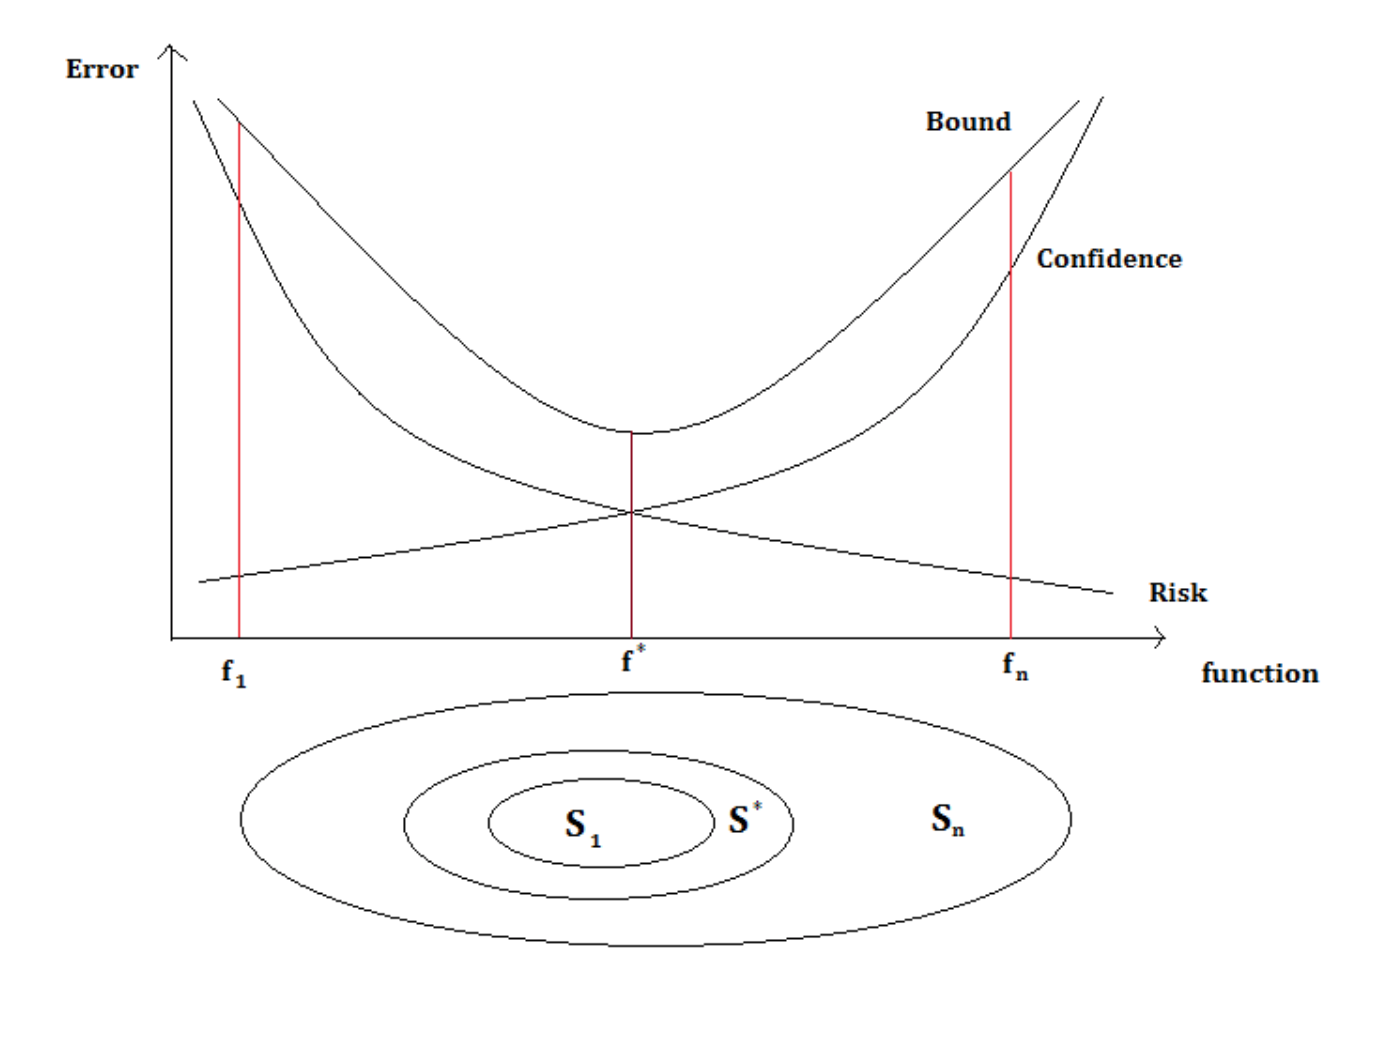
\includegraphics[scale=0.5]{structural_risk_minimization/SRMDiagram.png}
\caption{An illustration of the empirical risk and confidence for different functions. The optimal function is found at the minimum of the bound, listed as $f^{*}$}
\label{fig:srm}
\end{figure}

\index{structuralriskminimization|)}